\chapter{Implementation}
\label{chap:impl}

Chapter \ref{chap:related} points out that no real algorithm for stereoscopic video disparity yet exists.
Also, an evaluation suite that assesses disparity algorithms based on stereoscopic videos has not been build yet.
Datasets with high-resolution stereo videos are rarely available.
Source code for existing disparity algorithms are open-sourced and available for the public domain only in a few cases.
Additionally, a lot of different unaligned code for evaluation and comparing disparity is found.
Thus, the decision towards an implementation of a novel evaluation suite, built on top of OpenCV, was made.
Preexisting source code of disparity algorithms was refactored and integrated.
Different masks for fine-grained evaluation were implemented as well.
An image diminisher which alters stereo images by adding noise, to simulate real scenery, or artifacts from video compression was created.
Additionally, a web front-end was developed to present and visualize the results from any benchmark run within the suite.
\newline\newline\noindent The following sections describe the implementation, its components and the subsequent evaluation pipeline for disparity maps.
First, the preliminaries are outlined and an overview on the implementation as well as the evaluation engine is given.
Second, the integration of existing disparity algorithms is presented.
Third, the masks for the evaluation are explained and the implementation is described.
Fourth, the image diminisher, created to simulate real use cases is presented.
Finally, a simple stereo matcher which respects the spatiotemporal context is described in more detail and the web result viewer of the evaluation engine is introduced.

\section{Preliminaries}

As development platform a MacBookPro was used with the following specifications: i5-4258U CPU @ 2.40GHz (dual-core), 8 GB RAM, a fast SSD.
For the later evaluation phase a desktop computer with an i5-2500k @ 3.30GHz (quad-core) was considered.
The programming part was done with Atom\footnote{\url{https://atom.io}}, a modern text editor, and CLion\footnote{\url{https://www.jetbrains.com/clion/}} from JetBrains, a cross-platform IDE especially for C++.
CMake as a cross-compiling makefile generator was utilized.
Everything except the web result viewer was implemented using C++.
To reduce the effort of building an evaluation suite from scratch and for reducing code duplicates OpenCV was used.
The final build-chain consists of a set of shell scripts and CMake as makefile generator.
With CMake it was possible to cross-compile the app for Linux and use a fast server-instance from DigitalOcean\footnote{\url{https://www.digitalocean.com}} for the generation of the disparity maps and to actually evaluate those.
\newline\newline\noindent To not rely on different environments, docker images have been used to serve as basis for containerized virtual environments for the evaluation suite.
For this purpose, an image especially for OpenCV\footnote{\url{https://github.com/benjohnde/dockerbase-opencv}} was created, open-sourced and used.
Docker is a tool for the creation of containers and helps to build, run and ship distributed applications.
Those docker containers work in a chroot\footnote{Chroot stands for "change root" and helps to change the root directory for a current process.} environment and are isolated from other processes.
It is not a complete virtualized machine as it runs on the system's kernel.
Finally, the scripting language Python was used to create a set of scripts for combining all components in a chain.

\section{Overview}

Initially, a rapid monolithic prototype was built, featuring the execution of different disparity algorithms for each frame, the creation of masks and the evaluation of a given scene with different quality metrics.
But as more datasets were found and various masks as an evaluation method were implemented, the need for a leaner process chain arose.
Especially, as disparity algorithms need some time to compute the disparity map for one frame a more split approach was favored.
Hence, as videos consist of multiple frames (in our datasets about 100 frames in mean) this is a time consuming task.
Sometimes metrics change, the threshold is adjusted or a new metric is found.
As a result, the implementation consists of small services, with which computed disparity maps can be computed and evaluated independently.
Thus, the monolithic prototype was rewritten and partitioned in smaller microservices shaping three different components:

\begin{itemize}
  \item disparity algorithm executer,
  \item mask creator,
  \item evaluation engine.
\end{itemize}

\noindent Additionally, a small tool for diminishing images was created.
It can simulate real scenery by adding Gaussian noise as recommended by \citep{richardt2010real}.
In addition, FFmpeg \citep{FFMPEG2010} was wrapped to simulate artifacts originating from video compression.
The output, which each one of those microservices in the chain can generate or operate on, is structured in a simple folder tree.
\newline\newline\noindent The Figure \ref{fig:impl-pipeline} shows the composition and the evaluation chain of these services.
As described in the following subsections, the mask creator needs only the left image, as the disparity map is calculated for the left image as reference.
Thus, the masks are only created for the reference image.

\tikzstyle{rblock} = [text width=10em, rectangle, draw, fill=blue!20, text centered, rounded corners, minimum height=4em]
\tikzstyle{cloud} = [text width=6em, ellipse, draw, fill=red!15, text centered, rounded corners, minimum height=3.2em]
\begin{figure}[h!]
  \centering
  \scalebox{0.85}{
  \begin{tikzpicture}[node distance=7em, auto]
    %input
    \node [cloud] (right) {right image};
    \node [cloud, right of=right, node distance=10em] (left) {left image};
    \node [cloud, right of=left, node distance=10em] (disp) {ground-truth};

    %computation
    \node [rblock, below of=right, xshift=2em] (exec) {(1) Algorithm executer};
    \node [rblock, below of=disp, xshift=-2em] (mask-creator) {(2) Mask creator};
    
    %diminisher
    \node [rblock, above of=exec, yshift=7em] (dim) {(4) Image diminisher};

    %output
    \node [cloud, below of=exec] (map) {disparity map};
    \node [cloud, below of=mask-creator] (masks) {masks};

    %evaluation
    \node [rblock, below of=left, yshift=-14em] (evaluation) {(3) Disparity evaluator};

    %final result
    \node [cloud, below of=evaluation, xshift=-5em] (csv) {CSV file};
    \node [cloud, below of=evaluation, xshift=5em] (heatmaps) {heatmaps};

    %lines
    \path [line] (dim) -- (right);
    \path [line] (dim) -- (left);
    
    \path [line] (right) -- (exec);
    \path [line] (left) -- (exec);
    \path [line] (left) -- (mask-creator);
    \path [line] (disp) -- (mask-creator);

    \path [line] (exec) -- (map);
    \path [line] (mask-creator) -- (masks);

    \path [line] (map) -- (evaluation);
    \path [line] (masks) -- (evaluation);

    \path [line] (evaluation) -- (csv);
    \path [line] (evaluation) -- (heatmaps);
  \end{tikzpicture}
  }
  \caption{Composition and processing pipeline of the implementation.}
  \label{fig:impl-pipeline}
\end{figure}

\noindent In contrast to other implementations, input and output are clearly defined and thus different techniques can be adapted easily.
Combined frameworks which fulfill two tasks, disparity calculation (as the algorithm is implemented) and the final evaluation step exist.
This makes it harder to use the evaluation module separately from the rest.
None the less, the open source community around computer vision also lacks of code for a stereo matcher.
Due to the diversities of algorithms and evaluation suites, the decision was made to go for an OpenCV implementation of an eval suite for disparity algorithms.
\newline\newline\noindent At the current point in time, no disparity algorithms that directly target videos yet exist.
As a video is defined by multiple consecutive frames, every disparity algorithm for images can also be applied on videos.
The drawback of this trivial approach is the lack of taking the correlation of the frames into account.
None the less, it is possible to focus on some other details.
\newline\newline\noindent For instance, possible outliers in the sense of frames can occur, which may lead to more erroneous results.
The mean performance (error rate) of algorithms on a complete scene can be analyzed.
The runtime may vary in a sequence from frame-to-frame.
It is also interesting to see the impact of image diminishing effects like compression or noise, simulated as occurring from converting the signal from a real sensor.
This is described in greater detail in the upcoming section regarding image diminishing effects.
\newline\newline\noindent As middleware between the components OpenEXR\footnote{\url{http://www.openexr.com}} is used.
OpenEXR is a file format for high dynamic-range (HDR) images.
It supports 32-bit floating-point values and is thus good for representing sub-pixel accurate values in a disparity map.
The file format is also integrated in OpenCV.
For the later evaluation, the comparison of ground-truth data with computed disparity maps, it is sufficient.
However, to visualize the images on a default monitor, the values have to be normalized in a range suitable for using sophisticated color ranges like RGB.
Hence, heatmaps are created with normalized disparity maps in the range of $0-255$.
\newline\newline\noindent Basically, the evaluation engine takes a computed disparity map and the ground-truth counterpart as inputs.
Only comparing both provides low informative value.
Algorithms tend to produce disparity maps with a few unknown fields (e.g. noise or occluded pixels).
Crucial are also depth-discontinuities along object borders, textureless regions, and occluded pixels.
Thus, masks are used to only focus on these particular areas in an evaluation.
The creation of these masks are illustrated accurately in the upcoming section.
In Chapter \ref{chap:eval}, which discusses evaluation and results, the masks are used in combination with defined quality metrics.
The evaluation engine applies these quality metrics in combination with masks and outputs the result in a simple CSV file\footnote{CSV stands for comma-separated values. A CSV file usually represents a table, with rows being the lines and in columns the values are separated with commas.}.
As seen in Figure \ref{fig:impl-pipeline}, the implementation consists of three components.
After an algorithm is executed, the masks are created.
Finally, the computed disparity maps are compared with their ground-truth companion with each mask applied.
\newline\newline\noindent Python scripts in combination with the evaluation engine represent the whole eval-chain.
They work basically as a wrapper to iteratively execute each component over each frame of a given input sequence and aggregate the results.
The evaluation engine, as well as the other components, are run with command line arguments to pass specific parameters for the execution, for instance which input images should be used and where the computed disparity map should be saved.

\section{Integration of existing algorithms}

As shown in Chapter \ref{chap:related}, deciding which algorithms should be implemented was not easy.
There is a huge diversity of used technologies amongst disparity algorithms: various programming languages, CPU versus a CUDA\footnote{CUDA is a high level programming language that targets highly parallel calculations utilizing Graphic Processing Units (GPUs) by Nvidia.} implementation, different coding styles and libraries.
As a matter of fact, this makes it hard to implement and evaluate every available disparity algorithm.
Thus, a more streamlined extendable architecture is presented.
The algorithms, which were introduced in the related work Chapter \ref{chap:related}, are adopted and integrated.
The architecture of the disparity interface is depicted in Figure \ref{fig:uml-disparity-interface}.
\newline\newline\noindent The abstract class \texttt{DisparityAlgorithm} provides both images, left and right one, in form of a \texttt{cv::Mat} object and also holds the resulting disparity map.
On top of this abstract class further algorithms can be integrated easily.
The output of each algorithm is then saved in an OpenEXR file at a given destination path.
The following subsections describe how the algorithms were integrated, the pre- and post-processing steps if necessary, and illustrate the parameter.

\begin{figure}[h!]
  \centering
  \begin{tikzpicture}
    %classes
    \umlclass[x=2.5,y=8,type=abstract]{DisparityAlgorithm}{- left: cv::Mat\\- right: cv::Mat}{- compute()\\- setResult(mat: cv::Mat)}
    \umlclass[x=0,y=5.3]{ELASAlgorithm}{}{}
    \umlclass[x=4.5,y=5.3]{MRFStereo}{}{}
    \umlclass[x=2.5,y=3,type=interface]{OpenCVStereoMatcher}{}{}
    \umlclass[x=0,y=0]{OpenCVStereoBM}{}{}
    \umlclass[x=5,y=0]{OpenCVStereoSGBM}{}{}
    %connections
    \umluniassoc{OpenCVStereoMatcher}{DisparityAlgorithm}
    \umluniassoc{ELASAlgorithm}{DisparityAlgorithm}
    \umluniassoc{MRFStereo}{DisparityAlgorithm}
    \umlimpl{OpenCVStereoBM}{OpenCVStereoMatcher}
    \umlimpl{OpenCVStereoSGBM}{OpenCVStereoMatcher}
  \end{tikzpicture}
  \caption[Architectural overview on the disparity interface]{Architectural overview on the disparity interface in form of an UML diagram.}
  \label{fig:uml-disparity-interface}
\end{figure}

\subsection*{OpenCV}

The OpenCV library \citep{opencv_library}, currently at version 3.1.0, offers two implementations for disparity estimation, block matching and semi-global block matching based on the idea of \citeauthor{hirschmuller2005accurate} \citep{hirschmuller2005accurate}.
Both implementations are integrated and fed with the same input parameters.
The matching cost are calculated differently in both implementations.
Another difference is, that the simple block matching implementation only operates on grayscale.
As block size, an odd number needs to be used as adjacent pixels are observed.
Here, $9$ was chosen as block size.
A pre-filter was not used.
The speckle window, which is used to smooth disparities over noisy regions, is also not used.
The \texttt{disp12MaxDiff} parameter was set to $1$, which represents the maximum allowed difference in the left-to-right disparity consistency check.
If the difference is higher, the value is set as unknown.
The min- and max disparities are set to a value, which should be fit for most of the investigated sequences, $-48$ and $128$.
\newline\newline\noindent After an algorithm run, the disparity WLS filter is applied with $\lambda = 8000.0$ and $\sigma_{color} = 1.5$.
$\lambda$ defines the amount of regularization during the filtering process.
Larger values lead to over-smoothed edges in the disparity map, so that the disparity map adheres more to the source image edges.
$\sigma_{color}$ specifies how sensitive the filtering is done towards the source image edges.
Both are typical values for smoothing the disparity according to the OpenCV documentation.
As a post-processing step, the resulting \texttt{cv::Mat} has to be divided through $16$, as every input value gets multiplied with $16$ according to the source-code\footnote{\url{https://github.com/Itseez/opencv/blob/3942b1f36261b196a264e\\b35c996222848fe3c93/modules/calib3d/src/stereobm.cpp\#L564}}.
This step is integrated for sub-pixel-accurate disparity maps.
In the end, each point contains of 4 fractional bits.

\subsection*{Middlebury MRF library}

The Middlebury MRF library \citep{scharstein2006middlebury} consist of three parts, which all have to be composed together:
\begin{itemize}
  \item The imageLib, a small library for 2D multi-band images.
  \item MRF, an energy minimization software \citep{szeliski2008comparative}.
  \item mrfstereo, which is a stereo matcher front-end for the MRF library.
\end{itemize}

\noindent Some patches need to be applied to the MRF energy minimization software in order to get the graph cuts algorithms to work.
The composition is open-sourced\footnote{\url{https://github.com/benjohnde/disparity-algorithms}} with a Makefile.
Finally, a small wrapper for the execution was created.
The wrapper prepares the input images beforehand, saves them in a temporarily directory and post-processes the output.
The output is a disparity map, represented as 8-bit fixed points, where each disparity value has 4 fractional bits.
Thus, the result output is converted to a 32-bit floating values matrix, divided through $4$ and saved as OpenEXR file.
\newline\newline\noindent The MRF library offers the possibility to use the Birchfield-Tomasi method for matching cost calculation instead of the more commonly used sum of absolute differences (SAD).
\citeauthor{birchfield1999depth} defined matching cost as a global function which penalties occlusions and rewards matches \citep{birchfield1999depth}.
According to \citep{scharstein2002taxonomy, hirschmuller2007evaluation} the Birchfield-Tomasi method leads to better results than traditional similarities measurements like SAD.
In case of a traditional local similarities measurement, for instance SAD, it is possible to truncate the differences to a certain maximum value.
In Chapter \ref{chap:related}, the different algorithms, which are implemented in the Middlebury library, were presented.
The used algorithm can be selected via command-line parameter.
Other parameters are only for the smoothness term of the energy function.
It is possible to adjust the smoothness exponent, the maximum value of the smoothness term, and the weight $\lambda$ of the smoothness term.

\subsection*{ELAS: Efficient large-scaler stereo matching}

ELAS summarizes a front-end interface in combination with the library for efficient large-scale stereo matching (LIBELAS) from \citeauthor{Geiger2010ACCV} \citep{Geiger2010ACCV, Geiger2011IV}.
It offers a C++ library with a wrapper for MATLAB applications to compute disparity maps from rectified graylevel stereo pairs.
ELAS is integrated with a simple wrapper which executes the ELAS binary.
ELAS required the input files as PGM\footnote{PGM is a grayscale image format, part of the Netpbm library.} and outputs PFM\footnote{Similar to OpenEXR, PFM is a floating-point image file format, also part of the Netpbm library.} images.
In a preprocessing step the input stereo images are temporarily saved in the PGM format as grayscale images.
After the execution of ELAS, as a post-processing step, the PFM files are converted to OpenEXR files, as the subsequent processes expect OpenEXR files as input.
For processing the PFM files, a simple file reader was created, according to the official specifications\footnote{\url{http://netpbm.sourceforge.net/doc/pfm.html}}.
Specific characteristics of this file format are, that the rows are written bottom-to-top and each column has to be multiplied with a scale factor.
The ELAS binary can be started with no parameters but the maximum disparity value.

\section{Fine-grained evaluation via masks}

The trivial possibility for evaluation would be to just compare the computed disparity map with its ground-truth companion.
But, this approach would produce erroneous results due to a variety of reasons.
To give an example, occluded regions would lead to a higher error rate.
As a remedy, masks are introduced to simply focus on interesting pixels.
Masks are normal matrices of the size of the input image and they reflect two states: $0$ and $1$, whereas $1$ stands for masked.
In the literature they are sometimes also named bitmasks.
In this section the following masks are introduced:

\begin{itemize}
  \item depth-discontinuity,
  \item textured regions,
  \item occluded pixels,
  \item salient regions.
\end{itemize}

\noindent Programmatically they are represented through the OpenCV matrix class \texttt{cv::Mat} which can not work as a binary matrix and obtain just two states.
Thus, a \texttt{cv::Mat} with \texttt{CV\_8U1} is initialized, which means one color channel utilizing 8-bit unsigned for the values.
In this matrix, $1$ is mapped to $255$.

\subsection*{Depth-discontinuity}

Determining correspondence can fail in textureless or depth-discontinuous regions as mentioned beforehand in Chapter \ref{chap:foundations}.
Thus, it is interesting to see how disparity algorithms handle such regions.
So, a depth-discontinuity mask was implemented.
Depth-discontinuity is observed in the ground-truth disparity map.
It is defined as regions, where adjacent disparities differ by more than a certain gap \citep{scharstein2002taxonomy, cyganek2011introduction}.
For this purpose two basic morphological\footnote{Morphological operations are techniques to analyze and process geometrical structures.} image processing operations from the OpenCV library are used: \texttt{dilate} and \texttt{erode}.
\texttt{dilate} outputs for each position in a \texttt{cv::Mat} the maximum value of all the pixels in the neighborhood.
\texttt{erode} does nearly the same, but returns the minimum value.
Both are fed with a kernel, specifying which adjacent pixels should be taken into account.
\newline\newline\noindent For getting the disparity gap, the image gets dilated to get the maximum disparity of a pixel's neighbor.
Then eroded to estimate the minimum disparity of a pixel's neighbor.
Both is done with a $3x3$ kernel, and all adjacent pixels are masked to observe.
Finally, the depth-discontinuity areas are the ones with $maximum - truth > gap$.
The depth-discontinuity is then dilated by a window with given width to intense the area.
Visually, the best results are achieved with a gap of $2.0f$ and a width of $3$ for the final dilation.
Figure \ref{fig:dd-mask} depicts this.

\begin{figure}[h!]
\centering
\begin{tabular}{ccc}
\subfloat[ground-truth disparity]{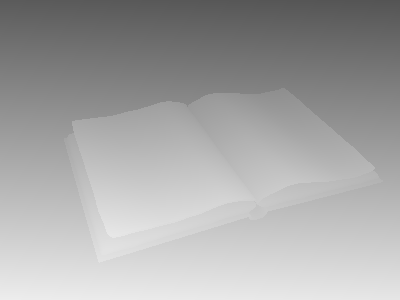
\includegraphics[width=0.3\textwidth]{src/images/book_ground-truth.png}} &
\subfloat[mask before final dilation]{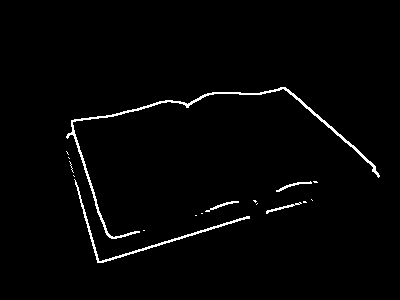
\includegraphics[width=0.3\textwidth]{src/images/book_dd_mask.png}} &
\subfloat[final mask for evaluation]{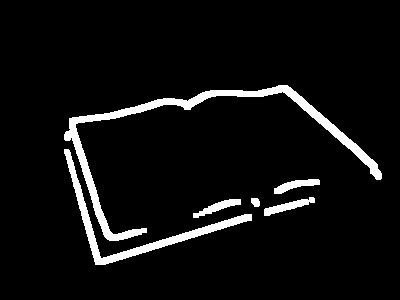
\includegraphics[width=0.3\textwidth]{src/images/book_dd_mask_final.png}}
\end{tabular}
\caption[Depth-discontinuity mask]{A depth-discontinuity mask, exampled with the first frame of the book scene from the Middlebury dataset.}
\label{fig:dd-mask}
\end{figure}

\subsection*{Textured regions}

Stereo matching algorithms act on the assumption, that disparity is smooth, especially if contrast and color intensity do not change drastically.
Therefore, it can be interesting to see how those algorithms treat textured and textureless regions.
Basically, regions with little or no texture in an image are defined as areas, where the squared horizontal intensity gradient, averaged over a square window of a given size, is below a given threshold \citep{scharstein2002taxonomy, cyganek2011introduction}.
\newline\newline\noindent This is implemented with the OpenCV \texttt{Sobel} operator and the \texttt{boxfilter}.
The sobel operator is a simple edge-detection filter which emphasizes edges in an image by representing the gradient magnitudes from the derivatives calculation.
The boxfilter is a blurring filter, which smoothes an image using a normalized kernel with a given size.
This is one of the simplest smoothing filters, as it just calculates the mean of its kernel neighbors, with all weighted equally.
So with the sobel filter, the edges are highlighted so that a computer can recognize them whereas the boxfilter smoothes the borders of recognized edges a bit.
Finally, the matrix of this outcome is checked against a threshold.
If a value of the matrix is greater than the threshold, the pixel is marked as a textured pixel.
\newline\newline\noindent The values for both, kernel size and threshold are depending of the scenery.
With the datasets which are evaluated in the upcoming Chapter \ref{chap:eval}, visually, the best results are achieved with a kernel size of $(2\ x\ 2)$ for the boxfilter, and a threshold of $16$.
Figure \ref{fig:textured-mask} depicts this approach.

\begin{figure}[h!]
\centering
\begin{tabular}{cc}
\subfloat[image of left camera]{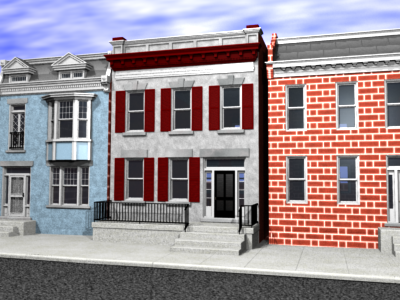
\includegraphics[width=0.45\textwidth]{src/images/street_left.png}} &
\subfloat[final textured mask]{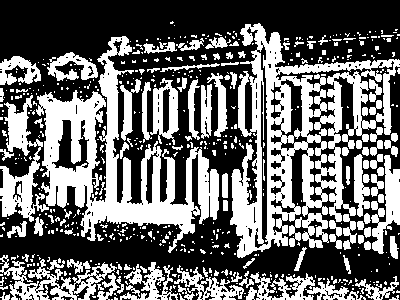
\includegraphics[width=0.45\textwidth]{src/images/street_textured_mask.png}}
\end{tabular}
\caption[Textured regions recognition]{Textured regions recognition with the first frame of the street scene from the Middlebury dataset.}
\label{fig:textured-mask}
\end{figure}

\subsection*{Occluded pixels}

An occluded pixel is defined as a pixel, which is hidden in one of the two images, for instance an object hides it from a different angle.
In the case of stereo matching the disparity can not be calculated for such pixels.
Thus, occluded pixels have to be handled properly, as they could distort our result.
For this purpose, a simple mask for non-occluded areas is introduced, to indicate which pixels on the scene are visible for both cameras and which are not.
Figure \ref{fig:noc-mask} shows an example of such a non-occluded areas mask.

\begin{figure}[h!]
\centering
\begin{tabular}{ccc}
\subfloat[left ground-truth]{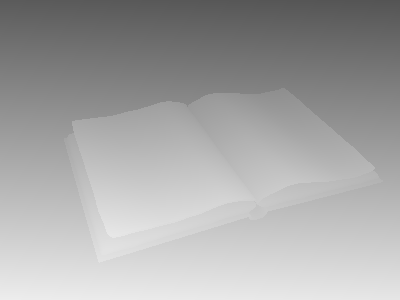
\includegraphics[width=0.3\textwidth]{src/images/book_ground-truth.png}} &
\subfloat[right ground-truth]{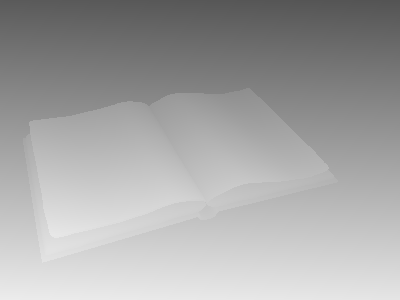
\includegraphics[width=0.3\textwidth]{src/images/book_ground-truth_right.png}} &
\subfloat[resulting mask]{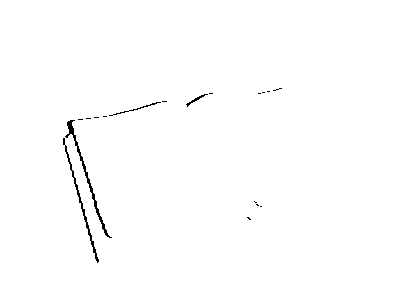
\includegraphics[width=0.3\textwidth]{src/images/book_noc_mask.png}}
\end{tabular}
\caption[Ground-truth disparity maps]{The ground-truth disparity maps of the first frame from the book scene is used to illustrate the non-occluded areas mask.}
\label{fig:noc-mask}
\end{figure}

\noindent To obtain the mask, both disparity maps, left and right one, are iterated.
Pixels that are visible from both cameras should have the same disparity value in both disparity maps.
For occluded pixels, the value is different \citep{scharstein2002taxonomy, martull2012realistic, cyganek2011introduction}.
Hence, a simple cross-check is sufficient.
It is implemented as the absolute value from the subtraction of the left value at a given position $d_L(x,y)$, and the right value at the corresponding position $d_R(x - d_L(x,y),y)$.
The result is then checked against a threshold.
If the value is greater than this threshold, the pixel is marked as occluded.
A suitable value for the threshold is $1$, according to \citep{scharstein2002taxonomy}.

\subsection*{Saliency detection}

As a novel approach, saliency detection is used as another criteria for the later evaluation.
There exist some algorithms for saliency detection in images and videos \citep{dittrich2013saliency, hou2007saliency, opencv_library}.
OpenCV offers two different saliency detection algorithms:
\begin{itemize}
  \item one for images, \texttt{StaticSaliency}, and
  \item one for videos \texttt{MotionSaliency}.
\end{itemize}

\noindent Here, the static saliency approach was used \citep{hou2007saliency} and implemented.
The algorithm outputs a saliency map with different saliency values, so a pixel can be more or less salient in the overall context.
This approach is also called the spectral residual approach as it analyzes the spectrum of an input image and creates a spectral residual model.
However, in the end a binary saliency map is outputted from the spectral residual model, where the pixels are masked as salient if their intensity in this spectral residual model is above a certain threshold.
This threshold can not be set as parameter, but is denoted as three times the average intensity of the saliency map.
Basically, the main idea is to extract the pixels which jump out of smooth curves, as they deserve most certainly the humans attention (cf. \citep{hou2007saliency}).
No parameters can be adjusted.
Figure \ref{fig:salient-mask} shows an example binary saliency map of an image from the SVDDD dataset, which will be presented in the upcoming Chapter \ref{chap:eval}.

\begin{figure}[h!]
\centering
\begin{tabular}{cc}
\subfloat[left image]{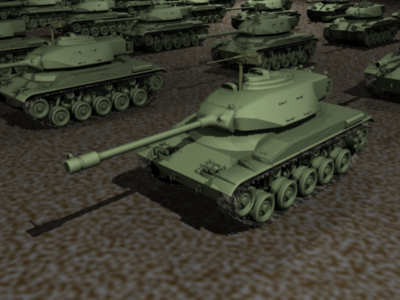
\includegraphics[width=0.45\textwidth]{src/images/tank-left.png}} &
\subfloat[salient mask]{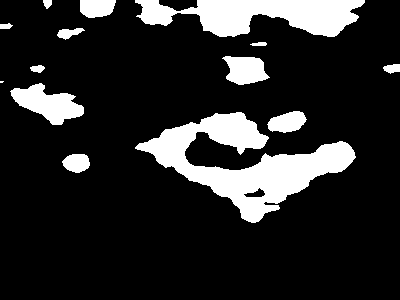
\includegraphics[width=0.45\textwidth]{src/images/tank-salient-mask.png}}
\end{tabular}
\caption[Saliency detection]{Frame of the tank sequence from the Cambridge dataset and the corresponding salient regions mask from the static saliency approach.}
\label{fig:salient-mask}
\end{figure}

\section{Image diminisher to simulate real use cases}

The presented masks can help to focus on different aspects during the evaluation.
Another interesting part of the evaluation is, to see the impact of small errors on the outcome of disparity algorithms.
For investigating the robustness of disparity algorithms against image diminishing effects like artifacts from video compression or noise like from a real sensor.
As both can be simulated by altering synthetic video sequences, an image diminisher to simulate real use cases is implemented.
Basically, this image diminisher consists of two parts: an OpenCV C++ program, which can add noise on top of images, and python script which wraps commands of FFmpeg to alter video sequences.

\tikzstyle{rblock} = [text width=8em, rectangle, draw, fill=blue!20, text centered, rounded corners, minimum height=4em]
\tikzstyle{cloud} = [text width=5em, ellipse, draw, fill=red!15, text centered, rounded corners, minimum height=3.2em]
\begin{figure}[h!]
  \vspace{1cm}
  \centering
  \begin{tikzpicture}[node distance=10em, auto]
    %nodes
    \node [cloud] (input) {input frame};
    \node [rblock, right of=input] (diminisher) {Image diminisher};
    \node [cloud, right of=diminisher] (output) {modified output frame};
    %lines
    \path [line] (input) -- (diminisher);
    \path [line] (diminisher) -- (output);
  \end{tikzpicture}
  \caption{Flow of the image diminisher.}
  \label{fig:image-diminisher-flow}
\end{figure}

\subsection*{Gaussian noise}

As seen in the related work in Chapter \ref{chap:related}, some approaches use restoration algorithms in order to reduce occurring noise.
Hence, noise generation was added as a preprocessing step in order to see how noise disrupts disparity algorithms in general.
Gaussian noise is used, meaning that the noise is Gaussian distributed (or normal distributed).
Normal (Gaussian) distribution is denoted as $\mathcal{N}(\mu,\sigma^2)$, where $\mu$ is the mean and $\sigma^2$ the variance (squared standard deviation).
\newline\newline\noindent As recommended by \citep{richardt2010real}, gaussian noise is added to synthetic video sequences with a mean of $0$ to simulate real scenery.
The variance, $\sigma^2$ can be set in our evaluation suite in order to see how this distracts the image.
\citeauthor{richardt2010real} recommended a variance of $20$.
The distribution is illustrated in Figure \ref{fig:gaussian}.
As can be seen, in comparison to $20$, a value of $5$ yields to modified pixels by adding values of $[-15;15]$.
Beforehand, to avoid errors, the matrix is converted from 8-bit to 16-bit in order to avoid overflow.
Finally, the matrix get reconverted to 8-bit.
Values $> 255$ and $< 0$ are fixed to $255$ and respectively $0$.
\newline\newline\noindent It is added with the \texttt{randn}\footnote{\url{http://docs.opencv.org/master/d2/de8/group__core__array.html\#gaeff1f61e972d133a04ce3a5f81cf6808}} function of the OpenCV library \citep{opencv_library}.
It generates a \texttt{cv::Mat} with the random distribution of values.
This matrix is then added on the source matrix, resulting in a noisy image.
For each frame, left and right, a new noise matrix is created.
Salt and pepper noise was not chosen, as it does not reflect real scenery.
Salt and pepper noise is not a common noise, as it contains random occurrences of black and white pixels.
It mostly appears by defect image sensors or erroneous analog-to-digital conversion.

\pgfmathdeclarefunction{gauss}{2}{%
  \pgfmathparse{1/(#2*sqrt(2*pi))*exp(-((x-#1)^2)/(2*#2^2))}%
}
\begin{figure}[h!]
  \vspace{1cm}
  \centering
  \begin{tikzpicture}
    \begin{axis}[every axis plot post/.append style={
      mark=none,domain=-16:+16,samples=50,smooth},
      axis x line*=bottom,
      axis y line*=left,
      enlargelimits=upper]
      \addplot {gauss(0,5)};
    \end{axis}
  \end{tikzpicture}
  \caption[Gaussian normal distribution]{Gaussian normal distribution with $\mathcal{N}(0,5)$.}
  \label{fig:gaussian}
\end{figure}

\subsection*{Video compression}

Most of the widely used video compression techniques belong to the lossy data compression algorithms.
As in contrast to lossless compression, lossy tends to produce small artifacts in images or videos as it does not reconstruct the original data as a whole.
FFmpeg \citep{FFMPEG2010} is used to simulate the degradation of stereo videos.
FFmpeg is a library for video en- and decoding to create video sequences from images with popular video codecs and also to divide a video sequences into images.
Figure \ref{fig:ffmpeg-flow} depicts the integration of FFmpeg in the image diminish process and how the python script invokes FFmpeg.
\newline\newline\noindent H.265\footnote{H.265 is also known as High Efficiency Video Coding (HEVC) and is a standard for encoding/decoding high-resolution video content.} was utilized as codec for video compression.
With H.265 only one parameter exists.
Here, FFmpeg is used with the libx265\footnote{\url{https://bitbucket.org/multicoreware/x265/overview}}, an open source HEVC encoder.
The only parameter, which can be set is the constant rate factor (CRF).
\newline\newline\noindent The CRF is a new technique to compress videos.
Normally, a quantizer scale factor (QP) exists in video compression.
This is a factor, which defines how strong the video should be compressed.
In traditional video compression techniques, this factor does not vary throughout a video and thus all frames receive the same compression.
H.265 as well as H.264 vary the QP according to the CRF depending on the scenery.
Fast moving scenes will receive a stronger QP than slow moving scenes, as the human eye will not focus on too many details in scenes with fast motion.
The suitable values vary from $0-51$, with $0$ implicating lossless compression and $51$ meaning the best possible compression with the worst visual outcome.
The default value is $28$ for H.265\footnote{\url{https://trac.ffmpeg.org/wiki/Encode/H.265}}.

\tikzstyle{rblock} = [text width=4em, rectangle, draw, fill=blue!20, text centered, rounded corners, minimum height=4em]
\tikzstyle{cloud} = [text width=6em, ellipse, draw, fill=red!15, text centered, rounded corners, minimum height=3.2em]
\begin{figure}[h!]
  \vspace{1cm}
  \centering
  \begin{tikzpicture}[node distance=9em, auto, scale=0.9, every node/.style={transform shape}]
    %nodes
    \node [cloud] (input) {set of stereo images};
    \node [rblock, right of=input] (ffmpeg1) {FFmpeg};
    \node [cloud, right of=ffmpeg1] (video1) {stereoscopic video};
    \node [rblock, right of=video1] (ffmpeg2) {FFmpeg};
    
    \node [cloud, below of=video1, yshift=2em] (video2) {compressed stereo video};
    \node [rblock, left of=video2] (ffmpeg3) {FFmpeg};
    \node [cloud, left of=ffmpeg3] (output) {set of diminished stereo images};
    %lines
    \path [line] (input) -- (ffmpeg1);
    \path [line] (ffmpeg1) -- (video1);
    \path [line] (video1) -- (ffmpeg2);
    
    \path [line] (ffmpeg2) -- node[anchor=north, xshift=-1.5em, yshift=1.0em] {H.265} (video2);
    \path [line] (video2) -- (ffmpeg3);
    \path [line] (ffmpeg3) -- (output);
  \end{tikzpicture}
  \caption{Flow of FFmpeg as image diminisher.}
  \label{fig:ffmpeg-flow}
\end{figure}

\section{Simple stereo matcher}

A simple naive stereo matcher (SNSM)\footnote{\url{https://github.com/benjohnde/disparity-evaluation/tree/master/4_NaiveImplementation}} has been implemented for several reasons.
First, the SNSM was built to see the limitations of such fast approaches without focusing for instance on arbitrary regions in an image, which can lead to erroneous results.
Second, to enhance the SNSM by adding the ability of taking the time axis into account, named spatiotemporal SNSM.
Third, to have a skeleton for further research and development.
It would be a tremendous task to implement a feature-complete stereo matcher, for instance implementing all available matching cost functions.
Hence, only the sum of absolute differences (SAD) was implemented as matching cost function.
Moreover, it is a simple area-matching approach with a given block (window) size.
Additionally, the previously introduced disparity constraints are not handled properly.
\newline\newline\noindent Algorithm \ref{alg:dsi-3d}, \textsc{CreateDisparitySpaceImage}, the matching cost for each possible disparity and stores them in a four-dimensional matrix.
As input parameter, the algorithm expects a set of rectified stereo image pairs, $I_L=\{I_{L_{1}}...I_{L_{n}}\}$ and $I_R=\{I_{R_{1}}...I_{R_{n}}\}$, whereas $n$ denotes the amount of images.
The maximum disparity to be found is denoted as $d_{max}$ whereas $wSize$ denotes the window size for the blocks to be matched.

\begin{algorithm}[h!]
\DontPrintSemicolon
\KwIn{$I_L$, $I_R$, $d_{max}$, $wSize$}
\KwOut{$C$}
$step \gets (wSize - 1) / 2$\;
$C \gets \textsc{CreateMatrix}(\textsc{Cols}(I_L),\textsc{Rows}(I_L),d_{max})$\;
$rows \gets \textsc{Rows}(I_L(0))$\;
$cols \gets \textsc{Cols}(I_L(0))$\;
$frames \gets \textsc{Images}(I_L)$\;
\For{$t \gets 0$ \textbf{to} $frames$} {
  $leftImage \gets I_L(t)$\;
  $rightImage \gets I_L(t)$\;
  \For{$y \gets 0 + step$ \textbf{to} $rows - step$} {
    \For{$x \gets 0 + step$ \textbf{to} $cols - step - d_{max}$} {
      \For{$d \gets 0$ \textbf{to} $d_{max}$} {
        $rect_{L} \gets \textsc{Rect}\{x - step, y - step, wSize, wSize\}$\;
        $rect_{R} \gets \textsc{Rect}\{x + d - step, y - step, wSize, wSize\}$\;
        $window_{L} \gets leftImage(rect_{L})$\;
        $window_{R} \gets rightImage(rect_{R})$\;
        $C(x,y,t,d) \gets \textsc{MatchingCost}(window_{L}, window_{R})$\;
      }
    }
  }
}
\Return{$C$}\;
\caption{\textsc{CreateDisparitySpaceImage}}
\label{alg:dsi-3d}
\end{algorithm}

\noindent $\textsc{Rect}\{x,y,width,height\}$ denotes a rectangle cropped out of a given image.
\textsc{CreateMatrix} creates a matrix with dimensions according to the input parameters.
The size of each dimension is defined with the parameter itself.
The output is the matrix $C = C(x,y,t,d)$ whereby $(x,y)$ is the position in the reference image $I_{L_{t}}$, $t$ the number of the frame and $d$ the disparity.
After the invocation, $C$ returns the matching cost for the given input.
\newline\newline\noindent Furthermore, the matching cost can be queried with the function $C(x,y,d) \iff C(x,y,0,d)$, which also represents the disparity space image, as introduced in the foundations Chapter \ref{chap:foundations}, by ignoring the time-dimension.
Algorithm \ref{alg:disparity-map}, \textsc{GetDisparityMap}, then computes the final disparity map by taking the disparity with the minimum matching cost for each field in the reference matrix.
$\textsc{Disparities}(C)$ outputs $d_{max}$, the length of the array holding the disparities, in this matrix.
\textsc{GetDisparityMap} needs as parameter the disparity space image, here denoted as $C(x,y,t,d)$ and the number of the frame $f$, for which the disparity map should be computed.
The matching cost is simply, as mentioned beforehand, the sum of absolute differences in a given window, as can be seen in Algorithm \ref{alg:matchingcost}, \textsc{MatchingCost}.
The $\Delta$ is estimated as the absolute difference between two windows.
Then, the cost is the sum of all fields in this matrix, which is computed by \textsc{MatrixSum}.
\newline\newline\noindent Algorithm \ref{alg:disparity-map} uses the Algorithm \ref{alg:best-match} which outputs the best match given an amount of disparities $d \in D=\{0{\dots}d_{max}\}$.
It iterates over all disparities and finds the minimum.
The best match is in this case the minimum matching cost.

\begin{algorithm}[h!]
\DontPrintSemicolon
\KwIn{$C$,}
\KwOut{$bestMatch$}
$disparities \gets \textsc{Disparities}(C)$\;
$cost \gets \infty$\;
$bestMatch \gets 0$\;
\For{$d \gets 0$ \textbf{to} $disparities$} {
  \If{$cost > C(d)$} {
    $cost \gets C(d)$\;
    $bestMatch \gets d$\;
  }
}
\Return{$bestMatch$}\;
\caption{\textsc{BestMatch}}
\label{alg:best-match}
\end{algorithm}

\noindent The spatiotemporal approach utilizes a new dimension, the time axis $t$, and adds it to the disparity space image.
$C(x,y,d,t)$ is constructed in Algorithm \ref{alg:dsi-3d} whereby $t \in T=\{0{\dots}n\}$ denotes the current processed frame.
Then, the DSI knows for each position, given a disparity and a frame the matching cost.
As a simple idea, the disparity, chosen for a frame, is the minimum over three frames.
Looking at a frame at time $f_t$, the frames $f_{t-1}$ and $f_{t+1}$ are also taken into account.
For the first and the last frame, the two following or respectively the two frames beforehand are used.
The underlying assumption is, that there is no much motion between the frames, because this would lead to inaccurate matching cost due to possible object hops.
\newline\newline\noindent If the amount of frames is smaller than three ($T < 3$), the spatiotemporal approach is not used.
Another possibility is to weight the frames.
Here, normal distribution was assumed.
Thus, the frame before and after the current frame are taken by $\frac{1}{4}$ into account, whereas the current frame is taken by $\frac{2}{4}$ into account.
As a result, a new matching cost matrix is created which reflects the disparity using the weighted approach.
The weighted approach can be toggled via the parameter $weighted$ in Algorithm \ref{alg:disparity-map}, which can be \textsc{True} or \textsc{False}.
For better representation, all approaches are integrated in Algorithm \ref{alg:disparity-map}.

\begin{algorithm}[h!]
\DontPrintSemicolon
\KwIn{$window_{L}$, $window_{R}$}
\KwOut{$cost$}
$\Delta \gets |window_{L} - window_{R}|$\;
$cost \gets \textsc{MatrixSum}(\Delta)$\;
\Return{$cost$}\;
\caption{\textsc{MatchingCost}}
\label{alg:matchingcost}
\end{algorithm}

\noindent Both, the unweighted and the weighted spatiotemporal approach are evaluated with the other introduced disparity algorithms.
The simple stereo matcher without the spatiotemporal dimension is evaluated as well.
The prediction is, that all three approaches get outperformed by the other stereo matcher.
The simple reason for that is the lack of handling the disparity constraints as described in the foundations Chapter \ref{chap:foundations}.
None the less, it is exciting to see, if the naive spatiotemporal approach achieves better results than without.
As of now, the weighted spatiotemporal approach is denoted as \textsc{WST-SNSM} whereas the unweighted approach is abbreviated as \textsc{UST-SNSM}.

\begin{algorithm}[h!]
\DontPrintSemicolon
\KwIn{$C$, $t$, $weighted$}
\KwOut{$DisparityMap$}
$DisparityMap \gets \textsc{CreateMatrix}(\textsc{Cols}(C),\textsc{Rows}(C))$\;
$step \gets (wSize - 1) / 2$\;
$rows \gets \textsc{Rows}(C)$\;
$cols \gets \textsc{Cols}(C)$\;
$frames \gets \textsc{Frames}(C)$\;
$disparities \gets \textsc{Disparities}(C)$\;
$spatiotemporal \gets frames < 3\ ?\ \textsc{True} : \textsc{False}$\;
\For{$t \gets 0$ \textbf{to} $frames$} {
  \For{$y \gets 0$ \textbf{to} $rows$} {
    \For{$x \gets 0$ \textbf{to} $cols$} {
      \If{$spatiotemporal == \textsc{True}$} {
        \If{$t == 0$} {
          $f_{0} \gets 0$\;
          $f_{1} \gets 1$\;
          $f_{2} \gets 2$\;
        }
        \ElseIf{$t == frames - 1$} {
          $f_{0} \gets frames - 3$\;
          $f_{1} \gets frames - 2$\;
          $f_{2} \gets frames - 1$\;
        }
        \Else {
          $f_{0} \gets t - 1$\;
          $f_{1} \gets t$\;
          $f_{2} \gets t + 1$\;
        }
        \If{$weighted == \textsc{True}$} {
          $Cost \gets \frac{1}{5} C(x,y,f_0) + \frac{2}{5} C(x,y,f_1)+ \frac{1}{5} C(x,y,f_2)$\;
        }
        \Else{
          $Cost \gets C(x,y,f_0) + C(x,y,f_1)+ C(x,y,f_2)$\;
        }
        $DisparityMap(x,y) \gets \textsc{BestMatch}(Cost)$\;
      }
      \Else {
        $DisparityMap(x,y) \gets \textsc{BestMatch}(C(x,y,f))$\;
      }
    }
  }
}
\Return{$DisparityMap$}\;
\caption{\textsc{GetDisparityMap}}
\label{alg:disparity-map}
\end{algorithm}

%explicit
\newpage

\section{Web result viewer of the evaluation suite}

As during the evaluation a lot of masks as well as heatmaps are created and saved, it was helpful to see the visual output of both, especially as a sequence of frames.
Thus, a web result viewer for the evaluation suite was implemented.
It was created with Node.js\footnote{Node.js is a framework for developing server-side web applications with JavaScript, cf. \url{https://nodejs.org/en/}.} and Express\footnote{Simple model-view-controller (MVC) web-framework, based on Node.js, cf. \url{http://expressjs.com}.}.
\newline\newline\noindent The following Figures \ref{fig:web-overview} and \ref{fig:web-detail} illustrate the implemented web result viewer.
The viewer displays all created masks and heatmaps, as well as the input images and their ground-truth disparity map.
In addition, an algorithm can be selected and the computed disparity map is shown.
The result is then visualized and the possibility to jump between frames as well as playing them automatically with different speed options is given.

\begin{figure}[h!]
  \centering
  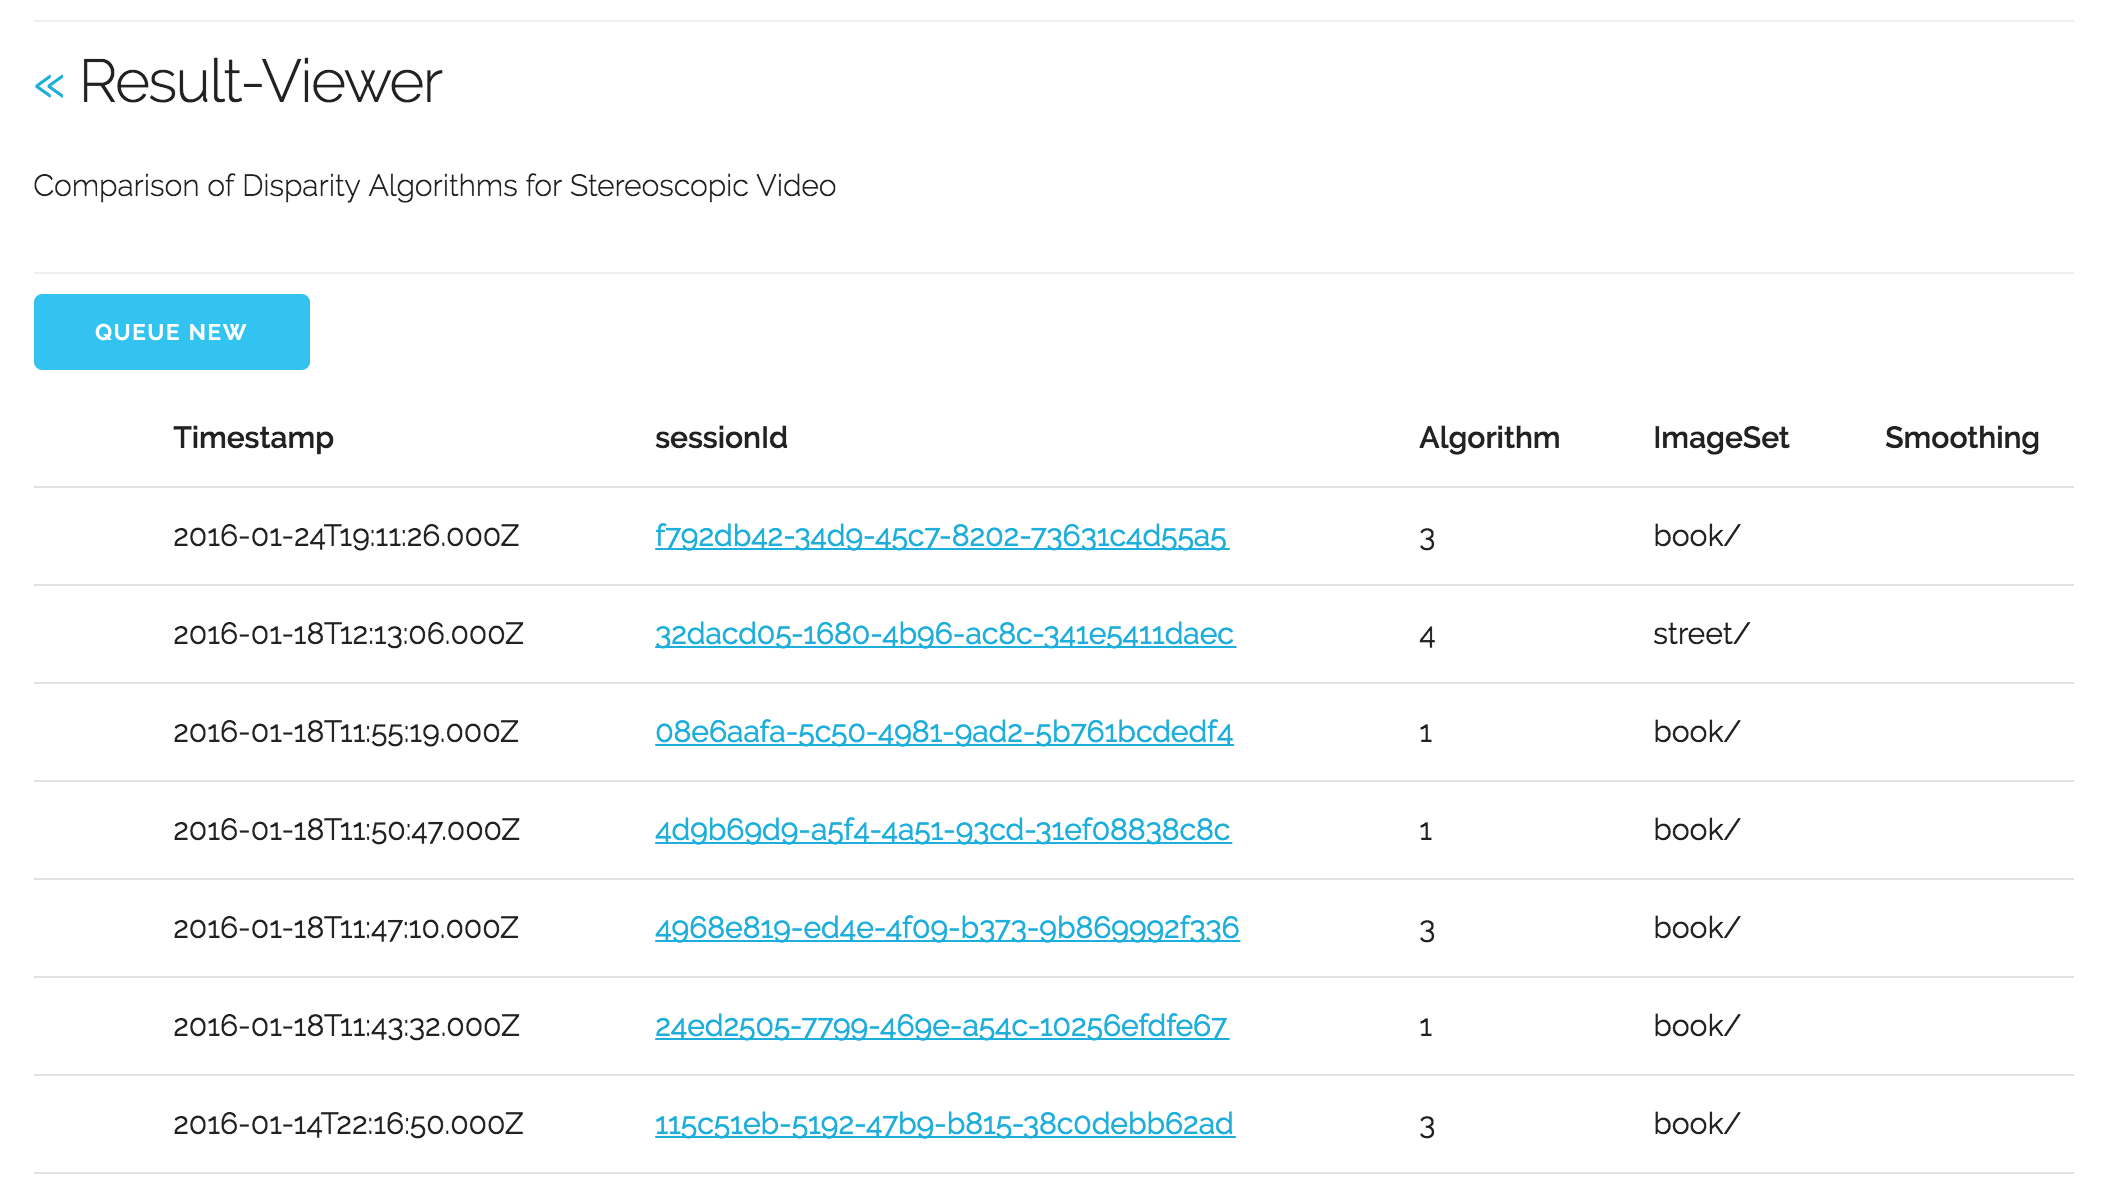
\includegraphics[width=1.0\textwidth]{src/images/result-viewer-overview.png}
  \caption[Overview page of the web result viewer]{Overview page of the web result viewer.}
  \label{fig:web-overview}
\end{figure}

\begin{figure}[p!]
  \centering
  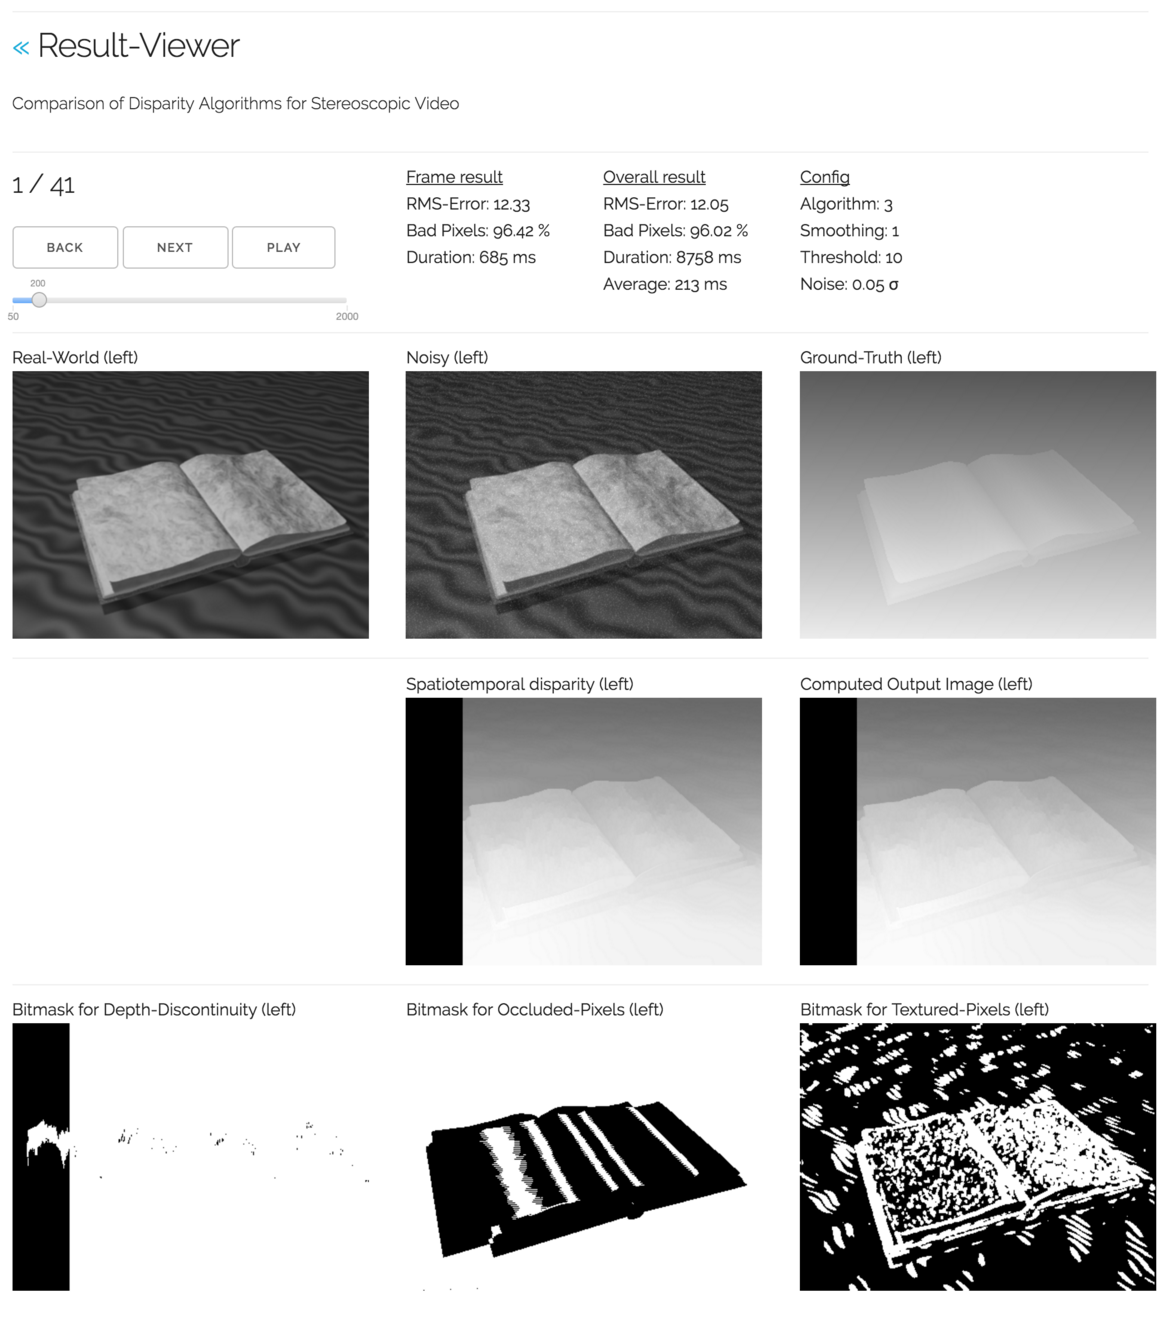
\includegraphics[width=1.0\textwidth]{src/images/result-viewer-detail.png}
  \caption{Detail of one result in the web result viewer.}
  \label{fig:web-detail}
\end{figure}
